\documentclass[twoside]{book}

% Packages required by doxygen
\usepackage{fixltx2e}
\usepackage{calc}
\usepackage{doxygen}
\usepackage[export]{adjustbox} % also loads graphicx
\usepackage{graphicx}
\usepackage[utf8]{inputenc}
\usepackage{makeidx}
\usepackage{multicol}
\usepackage{multirow}
\PassOptionsToPackage{warn}{textcomp}
\usepackage{textcomp}
\usepackage[nointegrals]{wasysym}
\usepackage[table]{xcolor}

% Font selection
\usepackage[T1]{fontenc}
\usepackage[scaled=.90]{helvet}
\usepackage{courier}
\usepackage{amssymb}
\usepackage{sectsty}
\renewcommand{\familydefault}{\sfdefault}
\allsectionsfont{%
  \fontseries{bc}\selectfont%
  \color{darkgray}%
}
\renewcommand{\DoxyLabelFont}{%
  \fontseries{bc}\selectfont%
  \color{darkgray}%
}
\newcommand{\+}{\discretionary{\mbox{\scriptsize$\hookleftarrow$}}{}{}}

% Page & text layout
\usepackage{geometry}
\geometry{%
  a4paper,%
  top=2.5cm,%
  bottom=2.5cm,%
  left=2.5cm,%
  right=2.5cm%
}
\tolerance=750
\hfuzz=15pt
\hbadness=750
\setlength{\emergencystretch}{15pt}
\setlength{\parindent}{0cm}
\setlength{\parskip}{3ex plus 2ex minus 2ex}
\makeatletter
\renewcommand{\paragraph}{%
  \@startsection{paragraph}{4}{0ex}{-1.0ex}{1.0ex}{%
    \normalfont\normalsize\bfseries\SS@parafont%
  }%
}
\renewcommand{\subparagraph}{%
  \@startsection{subparagraph}{5}{0ex}{-1.0ex}{1.0ex}{%
    \normalfont\normalsize\bfseries\SS@subparafont%
  }%
}
\makeatother

% Headers & footers
\usepackage{fancyhdr}
\pagestyle{fancyplain}
\fancyhead[LE]{\fancyplain{}{\bfseries\thepage}}
\fancyhead[CE]{\fancyplain{}{}}
\fancyhead[RE]{\fancyplain{}{\bfseries\leftmark}}
\fancyhead[LO]{\fancyplain{}{\bfseries\rightmark}}
\fancyhead[CO]{\fancyplain{}{}}
\fancyhead[RO]{\fancyplain{}{\bfseries\thepage}}
\fancyfoot[LE]{\fancyplain{}{}}
\fancyfoot[CE]{\fancyplain{}{}}
\fancyfoot[RE]{\fancyplain{}{\bfseries\scriptsize Generated by Doxygen }}
\fancyfoot[LO]{\fancyplain{}{\bfseries\scriptsize Generated by Doxygen }}
\fancyfoot[CO]{\fancyplain{}{}}
\fancyfoot[RO]{\fancyplain{}{}}
\renewcommand{\footrulewidth}{0.4pt}
\renewcommand{\chaptermark}[1]{%
  \markboth{#1}{}%
}
\renewcommand{\sectionmark}[1]{%
  \markright{\thesection\ #1}%
}

% Indices & bibliography
\usepackage{natbib}
\usepackage[titles]{tocloft}
\setcounter{tocdepth}{3}
\setcounter{secnumdepth}{5}
\makeindex

% Hyperlinks (required, but should be loaded last)
\usepackage{ifpdf}
\ifpdf
  \usepackage[pdftex,pagebackref=true]{hyperref}
\else
  \usepackage[ps2pdf,pagebackref=true]{hyperref}
\fi
\hypersetup{%
  colorlinks=true,%
  linkcolor=blue,%
  citecolor=blue,%
  unicode%
}

% Custom commands
\newcommand{\clearemptydoublepage}{%
  \newpage{\pagestyle{empty}\cleardoublepage}%
}

\usepackage{caption}
\captionsetup{labelsep=space,justification=centering,font={bf},singlelinecheck=off,skip=4pt,position=top}

%===== C O N T E N T S =====

\begin{document}

% Titlepage & ToC
\hypersetup{pageanchor=false,
             bookmarksnumbered=true,
             pdfencoding=unicode
            }
\pagenumbering{alph}
\begin{titlepage}
\vspace*{7cm}
\begin{center}%
{\Large G\+P\+ML \\[1ex]\large 0.\+1 }\\
\vspace*{1cm}
{\large Generated by Doxygen 1.8.13}\\
\end{center}
\end{titlepage}
\clearemptydoublepage
\pagenumbering{roman}
\tableofcontents
\clearemptydoublepage
\pagenumbering{arabic}
\hypersetup{pageanchor=true}

%--- Begin generated contents ---
\chapter{Class Index}
\section{Class List}
Here are the classes, structs, unions and interfaces with brief descriptions\+:\begin{DoxyCompactList}
\item\contentsline{section}{\hyperlink{classmath_1_1Matrix}{math\+::\+Matrix$<$ N $>$} \\*\hyperlink{classmath_1_1Matrix}{Matrix} generic class }{\pageref{classmath_1_1Matrix}}{}
\end{DoxyCompactList}

\chapter{File Index}
\section{File List}
Here is a list of all documented files with brief descriptions\+:\begin{DoxyCompactList}
\item\contentsline{section}{/home/daniel/dev/cpp/math/include/\hyperlink{Matrix_8hpp}{Matrix.\+hpp} }{\pageref{Matrix_8hpp}}{}
\item\contentsline{section}{/home/daniel/dev/cpp/math/include/\hyperlink{typedefs_8h}{typedefs.\+h} }{\pageref{typedefs_8h}}{}
\end{DoxyCompactList}

\chapter{Class Documentation}
\hypertarget{classmath_1_1Matrix}{}\section{math\+:\+:Matrix$<$ N $>$ Class Template Reference}
\label{classmath_1_1Matrix}\index{math\+::\+Matrix$<$ N $>$@{math\+::\+Matrix$<$ N $>$}}


\hyperlink{classmath_1_1Matrix}{Matrix} generic class.  




{\ttfamily \#include $<$Matrix.\+hpp$>$}

\subsection*{Public Member Functions}
\begin{DoxyCompactItemize}
\item 
\hyperlink{classmath_1_1Matrix_a766801644c0b1118db51d3d107daa732}{Matrix} (\hyperlink{typedefs_8h_a7b9b9413622e67b9df7f2d090b48682b}{uint} \hyperlink{classmath_1_1Matrix_ae99135c51efc0077b694ab37ad64d5c0}{size}, N fill)
\item 
\hyperlink{classmath_1_1Matrix_a0ba68b8b43efb8402dbecc0531df0bb5}{Matrix} (\hyperlink{typedefs_8h_a7b9b9413622e67b9df7f2d090b48682b}{uint} \hyperlink{classmath_1_1Matrix_a602173645d806afe305ed77b1ff38273}{rows}, \hyperlink{typedefs_8h_a7b9b9413622e67b9df7f2d090b48682b}{uint} \hyperlink{classmath_1_1Matrix_ad78b49e12a607856df124a18a855aaf1}{cols}, N fill)
\item 
\hyperlink{classmath_1_1Matrix_a24169476532305f1bb8229653274a5ba}{Matrix} (const \hyperlink{classmath_1_1Matrix}{Matrix} \&m)
\item 
N \hyperlink{classmath_1_1Matrix_aac510ef186a6bbf176d0ef4d79a7c666}{at} (\hyperlink{typedefs_8h_a7b9b9413622e67b9df7f2d090b48682b}{uint} r, \hyperlink{typedefs_8h_a7b9b9413622e67b9df7f2d090b48682b}{uint} c) const
\item 
void \hyperlink{classmath_1_1Matrix_afbf9ebd6114faec44e9eccb553ca8f33}{set} (\hyperlink{typedefs_8h_a7b9b9413622e67b9df7f2d090b48682b}{uint} r, \hyperlink{typedefs_8h_a7b9b9413622e67b9df7f2d090b48682b}{uint} c, N val)
\item 
std\+::pair$<$ \hyperlink{typedefs_8h_a7b9b9413622e67b9df7f2d090b48682b}{uint}, \hyperlink{typedefs_8h_a7b9b9413622e67b9df7f2d090b48682b}{uint} $>$ \hyperlink{classmath_1_1Matrix_afbbadd025c9d60f4447cee97fd7c727d}{shape} () const
\item 
\hyperlink{typedefs_8h_a7b9b9413622e67b9df7f2d090b48682b}{uint} \hyperlink{classmath_1_1Matrix_a602173645d806afe305ed77b1ff38273}{rows} () const
\item 
\hyperlink{typedefs_8h_a7b9b9413622e67b9df7f2d090b48682b}{uint} \hyperlink{classmath_1_1Matrix_ad78b49e12a607856df124a18a855aaf1}{cols} () const
\item 
\hyperlink{typedefs_8h_a7b9b9413622e67b9df7f2d090b48682b}{uint} \hyperlink{classmath_1_1Matrix_ae99135c51efc0077b694ab37ad64d5c0}{size} () const
\item 
\hyperlink{classmath_1_1Matrix}{Matrix} \& \hyperlink{classmath_1_1Matrix_a8bf5d371b703ef3023742c4058f709a7}{operator=} (const \hyperlink{classmath_1_1Matrix}{Matrix} \&m)
\item 
\hyperlink{classmath_1_1Matrix}{Matrix} \& \hyperlink{classmath_1_1Matrix_ae2944c1e1a0f1958101db2197bcfaa3c}{operator+=} (const \hyperlink{classmath_1_1Matrix}{Matrix} \&m)
\item 
\hyperlink{classmath_1_1Matrix}{Matrix} \& \hyperlink{classmath_1_1Matrix_a046b9f4717da34fb08795cb461497084}{operator-\/=} (const \hyperlink{classmath_1_1Matrix}{Matrix} \&m)
\item 
\hyperlink{classmath_1_1Matrix}{Matrix} \& \hyperlink{classmath_1_1Matrix_a1704c2b9fd200a6854b6793524a15700}{operator$\ast$=} (const N \&scal)
\item 
\hyperlink{classmath_1_1Matrix}{Matrix} \& \hyperlink{classmath_1_1Matrix_a4dbf1e0c5f42ce314ea2510a025b7e2a}{operator$\ast$=} (const \hyperlink{classmath_1_1Matrix}{Matrix} \&m)
\item 
\hyperlink{classmath_1_1Matrix}{Matrix} \& \hyperlink{classmath_1_1Matrix_a6a0a90575952ca84cac100cb40a5e9d0}{operator/=} (const N \&scal)
\item 
\hyperlink{classmath_1_1Matrix_afd52712eaef5a16115d605b7866a0576}{$\sim$\+Matrix} ()
\end{DoxyCompactItemize}


\subsection{Detailed Description}
\subsubsection*{template$<$typename N$>$\newline
class math\+::\+Matrix$<$ N $>$}

\hyperlink{classmath_1_1Matrix}{Matrix} generic class. 

\begin{DoxyAuthor}{Author}
Daniel Nichols 
\end{DoxyAuthor}
\begin{DoxyDate}{Date}
October 2018 
\end{DoxyDate}


\subsection{Constructor \& Destructor Documentation}
\mbox{\Hypertarget{classmath_1_1Matrix_a766801644c0b1118db51d3d107daa732}\label{classmath_1_1Matrix_a766801644c0b1118db51d3d107daa732}} 
\index{math\+::\+Matrix@{math\+::\+Matrix}!Matrix@{Matrix}}
\index{Matrix@{Matrix}!math\+::\+Matrix@{math\+::\+Matrix}}
\subsubsection{\texorpdfstring{Matrix()}{Matrix()}\hspace{0.1cm}{\footnotesize\ttfamily [1/3]}}
{\footnotesize\ttfamily template$<$typename N $>$ \\
\hyperlink{classmath_1_1Matrix}{math\+::\+Matrix}$<$ N $>$\+::\hyperlink{classmath_1_1Matrix}{Matrix} (\begin{DoxyParamCaption}\item[{\hyperlink{typedefs_8h_a7b9b9413622e67b9df7f2d090b48682b}{uint}}]{size,  }\item[{N}]{fill }\end{DoxyParamCaption})}

Square matrix constructor. Creates a size$\ast$size matrix with every value set to fill. 
\begin{DoxyParams}{Parameters}
{\em size} & -\/ size of the rows and cols of the matrix \\
\hline
{\em fill} & -\/ default value for every entry \\
\hline
\end{DoxyParams}
\mbox{\Hypertarget{classmath_1_1Matrix_a0ba68b8b43efb8402dbecc0531df0bb5}\label{classmath_1_1Matrix_a0ba68b8b43efb8402dbecc0531df0bb5}} 
\index{math\+::\+Matrix@{math\+::\+Matrix}!Matrix@{Matrix}}
\index{Matrix@{Matrix}!math\+::\+Matrix@{math\+::\+Matrix}}
\subsubsection{\texorpdfstring{Matrix()}{Matrix()}\hspace{0.1cm}{\footnotesize\ttfamily [2/3]}}
{\footnotesize\ttfamily template$<$typename N $>$ \\
\hyperlink{classmath_1_1Matrix}{math\+::\+Matrix}$<$ N $>$\+::\hyperlink{classmath_1_1Matrix}{Matrix} (\begin{DoxyParamCaption}\item[{\hyperlink{typedefs_8h_a7b9b9413622e67b9df7f2d090b48682b}{uint}}]{rows,  }\item[{\hyperlink{typedefs_8h_a7b9b9413622e67b9df7f2d090b48682b}{uint}}]{cols,  }\item[{N}]{fill }\end{DoxyParamCaption})}

\hyperlink{classmath_1_1Matrix}{Matrix} constructor. Creates a rows$\ast$cols matrix with every value set to fill. 
\begin{DoxyParams}{Parameters}
{\em rows} & -\/ number of rows \\
\hline
{\em cols} & -\/ number of cols \\
\hline
{\em fill} & -\/ default value for every entry \\
\hline
\end{DoxyParams}
\mbox{\Hypertarget{classmath_1_1Matrix_a24169476532305f1bb8229653274a5ba}\label{classmath_1_1Matrix_a24169476532305f1bb8229653274a5ba}} 
\index{math\+::\+Matrix@{math\+::\+Matrix}!Matrix@{Matrix}}
\index{Matrix@{Matrix}!math\+::\+Matrix@{math\+::\+Matrix}}
\subsubsection{\texorpdfstring{Matrix()}{Matrix()}\hspace{0.1cm}{\footnotesize\ttfamily [3/3]}}
{\footnotesize\ttfamily template$<$typename N $>$ \\
\hyperlink{classmath_1_1Matrix}{math\+::\+Matrix}$<$ N $>$\+::\hyperlink{classmath_1_1Matrix}{Matrix} (\begin{DoxyParamCaption}\item[{const \hyperlink{classmath_1_1Matrix}{Matrix}$<$ N $>$ \&}]{m }\end{DoxyParamCaption})}

Copy constructor. Copies matrix m into new matrix. 
\begin{DoxyParams}{Parameters}
{\em m} & -\/ matrix to be copied \\
\hline
\end{DoxyParams}
\mbox{\Hypertarget{classmath_1_1Matrix_afd52712eaef5a16115d605b7866a0576}\label{classmath_1_1Matrix_afd52712eaef5a16115d605b7866a0576}} 
\index{math\+::\+Matrix@{math\+::\+Matrix}!````~Matrix@{$\sim$\+Matrix}}
\index{````~Matrix@{$\sim$\+Matrix}!math\+::\+Matrix@{math\+::\+Matrix}}
\subsubsection{\texorpdfstring{$\sim$\+Matrix()}{~Matrix()}}
{\footnotesize\ttfamily template$<$typename N $>$ \\
\hyperlink{classmath_1_1Matrix}{math\+::\+Matrix}$<$ N $>$\+::$\sim$\hyperlink{classmath_1_1Matrix}{Matrix} (\begin{DoxyParamCaption}{ }\end{DoxyParamCaption})}

Destructor. Deletes the matrix internally 

\subsection{Member Function Documentation}
\mbox{\Hypertarget{classmath_1_1Matrix_aac510ef186a6bbf176d0ef4d79a7c666}\label{classmath_1_1Matrix_aac510ef186a6bbf176d0ef4d79a7c666}} 
\index{math\+::\+Matrix@{math\+::\+Matrix}!at@{at}}
\index{at@{at}!math\+::\+Matrix@{math\+::\+Matrix}}
\subsubsection{\texorpdfstring{at()}{at()}}
{\footnotesize\ttfamily template$<$typename N $>$ \\
N \hyperlink{classmath_1_1Matrix}{math\+::\+Matrix}$<$ N $>$\+::at (\begin{DoxyParamCaption}\item[{\hyperlink{typedefs_8h_a7b9b9413622e67b9df7f2d090b48682b}{uint}}]{r,  }\item[{\hyperlink{typedefs_8h_a7b9b9413622e67b9df7f2d090b48682b}{uint}}]{c }\end{DoxyParamCaption}) const}

Get element at r, c of the matrix 0-\/indexed. 
\begin{DoxyParams}{Parameters}
{\em r} & -\/ row of return element \\
\hline
{\em c} & -\/ column of return element \\
\hline
\end{DoxyParams}

\begin{DoxyExceptions}{Exceptions}
{\em invalid\+\_\+argument} & thrown if r$<$0 or r$>$=\hyperlink{classmath_1_1Matrix_a602173645d806afe305ed77b1ff38273}{rows()} or c$<$0 or c$>$=\hyperlink{classmath_1_1Matrix_ad78b49e12a607856df124a18a855aaf1}{cols()} \\
\hline
\end{DoxyExceptions}
\mbox{\Hypertarget{classmath_1_1Matrix_ad78b49e12a607856df124a18a855aaf1}\label{classmath_1_1Matrix_ad78b49e12a607856df124a18a855aaf1}} 
\index{math\+::\+Matrix@{math\+::\+Matrix}!cols@{cols}}
\index{cols@{cols}!math\+::\+Matrix@{math\+::\+Matrix}}
\subsubsection{\texorpdfstring{cols()}{cols()}}
{\footnotesize\ttfamily template$<$typename N$>$ \\
\hyperlink{typedefs_8h_a7b9b9413622e67b9df7f2d090b48682b}{uint} \hyperlink{classmath_1_1Matrix}{math\+::\+Matrix}$<$ N $>$\+::cols (\begin{DoxyParamCaption}{ }\end{DoxyParamCaption}) const\hspace{0.3cm}{\ttfamily [inline]}}

Get the number of columns in the matrix. \begin{DoxyReturn}{Returns}
the number of columns in the matrix 
\end{DoxyReturn}
\mbox{\Hypertarget{classmath_1_1Matrix_a1704c2b9fd200a6854b6793524a15700}\label{classmath_1_1Matrix_a1704c2b9fd200a6854b6793524a15700}} 
\index{math\+::\+Matrix@{math\+::\+Matrix}!operator$\ast$=@{operator$\ast$=}}
\index{operator$\ast$=@{operator$\ast$=}!math\+::\+Matrix@{math\+::\+Matrix}}
\subsubsection{\texorpdfstring{operator$\ast$=()}{operator*=()}\hspace{0.1cm}{\footnotesize\ttfamily [1/2]}}
{\footnotesize\ttfamily template$<$typename N $>$ \\
\hyperlink{classmath_1_1Matrix}{Matrix}$<$ N $>$ \& \hyperlink{classmath_1_1Matrix}{math\+::\+Matrix}$<$ N $>$\+::operator$\ast$= (\begin{DoxyParamCaption}\item[{const N \&}]{scal }\end{DoxyParamCaption})}

Adds Multiplies {\ttfamily this} by scaler {\ttfamily scal} 
\begin{DoxyParams}{Parameters}
{\em scal} & -\/ scaler to multiply {\ttfamily this} by \\
\hline
\end{DoxyParams}
\begin{DoxyReturn}{Returns}
a pointer to {\ttfamily m} after multiplication 
\end{DoxyReturn}
\mbox{\Hypertarget{classmath_1_1Matrix_a4dbf1e0c5f42ce314ea2510a025b7e2a}\label{classmath_1_1Matrix_a4dbf1e0c5f42ce314ea2510a025b7e2a}} 
\index{math\+::\+Matrix@{math\+::\+Matrix}!operator$\ast$=@{operator$\ast$=}}
\index{operator$\ast$=@{operator$\ast$=}!math\+::\+Matrix@{math\+::\+Matrix}}
\subsubsection{\texorpdfstring{operator$\ast$=()}{operator*=()}\hspace{0.1cm}{\footnotesize\ttfamily [2/2]}}
{\footnotesize\ttfamily template$<$typename N $>$ \\
\hyperlink{classmath_1_1Matrix}{Matrix}$<$ N $>$ \& \hyperlink{classmath_1_1Matrix}{math\+::\+Matrix}$<$ N $>$\+::operator$\ast$= (\begin{DoxyParamCaption}\item[{const \hyperlink{classmath_1_1Matrix}{Matrix}$<$ N $>$ \&}]{m }\end{DoxyParamCaption})}

Performs matrix multiplication between {\ttfamily this} and {\ttfamily m}. This operation will throw an exception if {\ttfamily cols!=m.\+rows()}. It will also reshape {\ttfamily this} to that {\ttfamily \hyperlink{classmath_1_1Matrix_a602173645d806afe305ed77b1ff38273}{rows()}} does not change and {\ttfamily \hyperlink{classmath_1_1Matrix_ad78b49e12a607856df124a18a855aaf1}{cols()}} becomes {\ttfamily m.\+cols()}. 
\begin{DoxyParams}{Parameters}
{\em m} & -\/ matrix to multiply by {\ttfamily this}. \\
\hline
\end{DoxyParams}
\begin{DoxyReturn}{Returns}
a pointer to {\ttfamily this} after multiplication. 
\end{DoxyReturn}

\begin{DoxyExceptions}{Exceptions}
{\em invalid\+\_\+argument} & if {\ttfamily \hyperlink{classmath_1_1Matrix_ad78b49e12a607856df124a18a855aaf1}{cols()}!=m.\+rows()} matrix multiplication is undefined \\
\hline
\end{DoxyExceptions}
\mbox{\Hypertarget{classmath_1_1Matrix_ae2944c1e1a0f1958101db2197bcfaa3c}\label{classmath_1_1Matrix_ae2944c1e1a0f1958101db2197bcfaa3c}} 
\index{math\+::\+Matrix@{math\+::\+Matrix}!operator+=@{operator+=}}
\index{operator+=@{operator+=}!math\+::\+Matrix@{math\+::\+Matrix}}
\subsubsection{\texorpdfstring{operator+=()}{operator+=()}}
{\footnotesize\ttfamily template$<$typename N $>$ \\
\hyperlink{classmath_1_1Matrix}{Matrix}$<$ N $>$ \& \hyperlink{classmath_1_1Matrix}{math\+::\+Matrix}$<$ N $>$\+::operator+= (\begin{DoxyParamCaption}\item[{const \hyperlink{classmath_1_1Matrix}{Matrix}$<$ N $>$ \&}]{m }\end{DoxyParamCaption})}

Adds matrix {\ttfamily m} to {\ttfamily this} element-\/wise 
\begin{DoxyParams}{Parameters}
{\em m} & -\/ matrix to add to {\ttfamily this}. rows and cols must be equivalent. \\
\hline
\end{DoxyParams}
\begin{DoxyReturn}{Returns}
a pointer to {\ttfamily this} after addition 
\end{DoxyReturn}

\begin{DoxyExceptions}{Exceptions}
{\em invalid\+\_\+argument} & thrown if {\ttfamily \hyperlink{classmath_1_1Matrix_a602173645d806afe305ed77b1ff38273}{rows()}!=m.\+rows()} or {\ttfamily \hyperlink{classmath_1_1Matrix_ad78b49e12a607856df124a18a855aaf1}{cols()}!=m.\+cols()} \\
\hline
\end{DoxyExceptions}
\mbox{\Hypertarget{classmath_1_1Matrix_a046b9f4717da34fb08795cb461497084}\label{classmath_1_1Matrix_a046b9f4717da34fb08795cb461497084}} 
\index{math\+::\+Matrix@{math\+::\+Matrix}!operator-\/=@{operator-\/=}}
\index{operator-\/=@{operator-\/=}!math\+::\+Matrix@{math\+::\+Matrix}}
\subsubsection{\texorpdfstring{operator-\/=()}{operator-=()}}
{\footnotesize\ttfamily template$<$typename N $>$ \\
\hyperlink{classmath_1_1Matrix}{Matrix}$<$ N $>$ \& \hyperlink{classmath_1_1Matrix}{math\+::\+Matrix}$<$ N $>$\+::operator-\/= (\begin{DoxyParamCaption}\item[{const \hyperlink{classmath_1_1Matrix}{Matrix}$<$ N $>$ \&}]{m }\end{DoxyParamCaption})}

Subtracts matrix {\ttfamily m} from {\ttfamily this} element-\/wise 
\begin{DoxyParams}{Parameters}
{\em m} & -\/ matrix to subtract from {\ttfamily this}. rows and cols must be equivalent. \\
\hline
\end{DoxyParams}
\begin{DoxyReturn}{Returns}
a pointer to {\ttfamily this} after subtraction 
\end{DoxyReturn}

\begin{DoxyExceptions}{Exceptions}
{\em invalid\+\_\+argument} & thrown if {\ttfamily \hyperlink{classmath_1_1Matrix_a602173645d806afe305ed77b1ff38273}{rows()}!=m.\+rows()} or {\ttfamily \hyperlink{classmath_1_1Matrix_ad78b49e12a607856df124a18a855aaf1}{cols()}!=m.\+cols()} \\
\hline
\end{DoxyExceptions}
\mbox{\Hypertarget{classmath_1_1Matrix_a6a0a90575952ca84cac100cb40a5e9d0}\label{classmath_1_1Matrix_a6a0a90575952ca84cac100cb40a5e9d0}} 
\index{math\+::\+Matrix@{math\+::\+Matrix}!operator/=@{operator/=}}
\index{operator/=@{operator/=}!math\+::\+Matrix@{math\+::\+Matrix}}
\subsubsection{\texorpdfstring{operator/=()}{operator/=()}}
{\footnotesize\ttfamily template$<$typename N$>$ \\
\hyperlink{classmath_1_1Matrix}{Matrix}\& \hyperlink{classmath_1_1Matrix}{math\+::\+Matrix}$<$ N $>$\+::operator/= (\begin{DoxyParamCaption}\item[{const N \&}]{scal }\end{DoxyParamCaption})}

Divides {\ttfamily this} by scalar {\ttfamily scal} element-\/wise. Does not check for {\ttfamily scal==0} as division for class {\ttfamily N} might have non-\/standard definition. 
\begin{DoxyParams}{Parameters}
{\em scal} & -\/ scalar to divide {\ttfamily this} by \\
\hline
\end{DoxyParams}
\begin{DoxyReturn}{Returns}
a pointer to {\ttfamily m} after division 
\end{DoxyReturn}
\mbox{\Hypertarget{classmath_1_1Matrix_a8bf5d371b703ef3023742c4058f709a7}\label{classmath_1_1Matrix_a8bf5d371b703ef3023742c4058f709a7}} 
\index{math\+::\+Matrix@{math\+::\+Matrix}!operator=@{operator=}}
\index{operator=@{operator=}!math\+::\+Matrix@{math\+::\+Matrix}}
\subsubsection{\texorpdfstring{operator=()}{operator=()}}
{\footnotesize\ttfamily template$<$typename N $>$ \\
\hyperlink{classmath_1_1Matrix}{Matrix}$<$ N $>$ \& \hyperlink{classmath_1_1Matrix}{math\+::\+Matrix}$<$ N $>$\+::operator= (\begin{DoxyParamCaption}\item[{const \hyperlink{classmath_1_1Matrix}{Matrix}$<$ N $>$ \&}]{m }\end{DoxyParamCaption})}

Copies {\ttfamily m} into {\ttfamily this}. Performs an element-\/wise copy. Ignores self-\/copy. 
\begin{DoxyParams}{Parameters}
{\em m} & -\/ matrix to copy into {\ttfamily this} \\
\hline
\end{DoxyParams}
\begin{DoxyReturn}{Returns}
pointer to {\ttfamily this} after copy 
\end{DoxyReturn}
\mbox{\Hypertarget{classmath_1_1Matrix_a602173645d806afe305ed77b1ff38273}\label{classmath_1_1Matrix_a602173645d806afe305ed77b1ff38273}} 
\index{math\+::\+Matrix@{math\+::\+Matrix}!rows@{rows}}
\index{rows@{rows}!math\+::\+Matrix@{math\+::\+Matrix}}
\subsubsection{\texorpdfstring{rows()}{rows()}}
{\footnotesize\ttfamily template$<$typename N$>$ \\
\hyperlink{typedefs_8h_a7b9b9413622e67b9df7f2d090b48682b}{uint} \hyperlink{classmath_1_1Matrix}{math\+::\+Matrix}$<$ N $>$\+::rows (\begin{DoxyParamCaption}{ }\end{DoxyParamCaption}) const\hspace{0.3cm}{\ttfamily [inline]}}

Get the number of rows in the matrix. \begin{DoxyReturn}{Returns}
the number of rows in the matrix 
\end{DoxyReturn}
\mbox{\Hypertarget{classmath_1_1Matrix_afbf9ebd6114faec44e9eccb553ca8f33}\label{classmath_1_1Matrix_afbf9ebd6114faec44e9eccb553ca8f33}} 
\index{math\+::\+Matrix@{math\+::\+Matrix}!set@{set}}
\index{set@{set}!math\+::\+Matrix@{math\+::\+Matrix}}
\subsubsection{\texorpdfstring{set()}{set()}}
{\footnotesize\ttfamily template$<$typename N $>$ \\
void \hyperlink{classmath_1_1Matrix}{math\+::\+Matrix}$<$ N $>$\+::set (\begin{DoxyParamCaption}\item[{\hyperlink{typedefs_8h_a7b9b9413622e67b9df7f2d090b48682b}{uint}}]{r,  }\item[{\hyperlink{typedefs_8h_a7b9b9413622e67b9df7f2d090b48682b}{uint}}]{c,  }\item[{N}]{val }\end{DoxyParamCaption})}

Set element at r, c of the matrix 0-\/indexed. 
\begin{DoxyParams}{Parameters}
{\em r} & -\/ row of element set \\
\hline
{\em c} & -\/ column of element set \\
\hline
{\em val} & -\/ value to set element at r,c \\
\hline
\end{DoxyParams}

\begin{DoxyExceptions}{Exceptions}
{\em invalid\+\_\+argument} & thrown if r$<$0 or r$>$=\hyperlink{classmath_1_1Matrix_a602173645d806afe305ed77b1ff38273}{rows()} or c$<$0 or c$>$=\hyperlink{classmath_1_1Matrix_ad78b49e12a607856df124a18a855aaf1}{cols()} \\
\hline
\end{DoxyExceptions}
\mbox{\Hypertarget{classmath_1_1Matrix_afbbadd025c9d60f4447cee97fd7c727d}\label{classmath_1_1Matrix_afbbadd025c9d60f4447cee97fd7c727d}} 
\index{math\+::\+Matrix@{math\+::\+Matrix}!shape@{shape}}
\index{shape@{shape}!math\+::\+Matrix@{math\+::\+Matrix}}
\subsubsection{\texorpdfstring{shape()}{shape()}}
{\footnotesize\ttfamily template$<$typename N$>$ \\
std\+::pair$<$\hyperlink{typedefs_8h_a7b9b9413622e67b9df7f2d090b48682b}{uint}, \hyperlink{typedefs_8h_a7b9b9413622e67b9df7f2d090b48682b}{uint}$>$ \hyperlink{classmath_1_1Matrix}{math\+::\+Matrix}$<$ N $>$\+::shape (\begin{DoxyParamCaption}{ }\end{DoxyParamCaption}) const\hspace{0.3cm}{\ttfamily [inline]}}

Get the shape or (rows, cols). This is equivalent to {\ttfamily std\+::make\+\_\+pair(\hyperlink{classmath_1_1Matrix_a602173645d806afe305ed77b1ff38273}{rows()}, \hyperlink{classmath_1_1Matrix_ad78b49e12a607856df124a18a855aaf1}{cols()});} \begin{DoxyReturn}{Returns}
an S\+TL pair containing the row count and column count 
\end{DoxyReturn}
\mbox{\Hypertarget{classmath_1_1Matrix_ae99135c51efc0077b694ab37ad64d5c0}\label{classmath_1_1Matrix_ae99135c51efc0077b694ab37ad64d5c0}} 
\index{math\+::\+Matrix@{math\+::\+Matrix}!size@{size}}
\index{size@{size}!math\+::\+Matrix@{math\+::\+Matrix}}
\subsubsection{\texorpdfstring{size()}{size()}}
{\footnotesize\ttfamily template$<$typename N$>$ \\
\hyperlink{typedefs_8h_a7b9b9413622e67b9df7f2d090b48682b}{uint} \hyperlink{classmath_1_1Matrix}{math\+::\+Matrix}$<$ N $>$\+::size (\begin{DoxyParamCaption}{ }\end{DoxyParamCaption}) const\hspace{0.3cm}{\ttfamily [inline]}}

Get the size of the matrix ({\ttfamily \hyperlink{classmath_1_1Matrix_ae99135c51efc0077b694ab37ad64d5c0}{size()} == \hyperlink{classmath_1_1Matrix_a602173645d806afe305ed77b1ff38273}{rows()} $\ast$ \hyperlink{classmath_1_1Matrix_ad78b49e12a607856df124a18a855aaf1}{cols()}}) \begin{DoxyReturn}{Returns}
the size of the matrix 
\end{DoxyReturn}


The documentation for this class was generated from the following file\+:\begin{DoxyCompactItemize}
\item 
/home/daniel/dev/cpp/math/include/\hyperlink{Matrix_8hpp}{Matrix.\+hpp}\end{DoxyCompactItemize}

\chapter{File Documentation}
\hypertarget{Matrix_8hpp}{}\section{/home/daniel/dev/cpp/math/include/\+Matrix.hpp File Reference}
\label{Matrix_8hpp}\index{/home/daniel/dev/cpp/math/include/\+Matrix.\+hpp@{/home/daniel/dev/cpp/math/include/\+Matrix.\+hpp}}
{\ttfamily \#include $<$utility$>$}\newline
{\ttfamily \#include $<$stdexcept$>$}\newline
{\ttfamily \#include \char`\"{}typedefs.\+h\char`\"{}}\newline
Include dependency graph for Matrix.\+hpp\+:\nopagebreak
\begin{figure}[H]
\begin{center}
\leavevmode
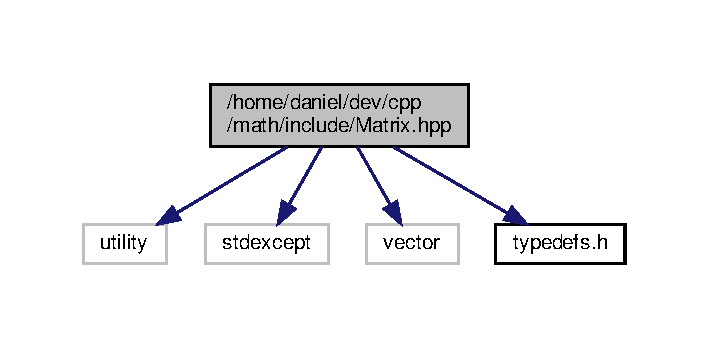
\includegraphics[width=278pt]{Matrix_8hpp__incl}
\end{center}
\end{figure}
\subsection*{Classes}
\begin{DoxyCompactItemize}
\item 
class \hyperlink{classmath_1_1Matrix}{math\+::\+Matrix$<$ N $>$}
\begin{DoxyCompactList}\small\item\em \hyperlink{classmath_1_1Matrix}{Matrix} generic class. \end{DoxyCompactList}\end{DoxyCompactItemize}
\subsection*{Typedefs}
\begin{DoxyCompactItemize}
\item 
typedef Matrix$<$ int $>$ \hyperlink{Matrix_8hpp_a09ee7d97ee3fb530f80cac82780711f8}{math\+::i\+Matrix}
\item 
typedef Matrix$<$ float $>$ \hyperlink{Matrix_8hpp_adb88834810480e2f18cf3d74a3954311}{math\+::f\+Matrix}
\item 
typedef Matrix$<$ double $>$ \hyperlink{Matrix_8hpp_a65b4179533da3857354550916c3ef90b}{math\+::d\+Matrix}
\end{DoxyCompactItemize}
\subsection*{Functions}
\begin{DoxyCompactItemize}
\item 
{\footnotesize template$<$typename N $>$ }\\Matrix$<$ N $>$ \hyperlink{Matrix_8hpp_a6e8f7c0c49b91a302a3c98c764d1bcf8}{math\+::operator+} (Matrix$<$ N $>$ lhs, const Matrix$<$ N $>$ \&rhs)
\item 
{\footnotesize template$<$typename N $>$ }\\Matrix$<$ N $>$ \hyperlink{Matrix_8hpp_a9bd8120f9bdad37a57f74aa4bbfcde67}{math\+::operator-\/} (Matrix$<$ N $>$ lhs, const Matrix$<$ N $>$ \&rhs)
\item 
{\footnotesize template$<$typename N $>$ }\\Matrix$<$ N $>$ \hyperlink{Matrix_8hpp_a8b2b9bc6e9c45e33a535f7b1650bc906}{math\+::operator$\ast$} (Matrix$<$ N $>$ lhs, const N \&rhs)
\item 
{\footnotesize template$<$typename N $>$ }\\Matrix$<$ N $>$ \hyperlink{Matrix_8hpp_a990777f6ce4e2deb13a59f23622fd8bc}{math\+::operator$\ast$} (const N \&lhs, Matrix$<$ N $>$ rhs)
\item 
{\footnotesize template$<$typename N $>$ }\\Matrix$<$ N $>$ \hyperlink{Matrix_8hpp_a66c4aedee806ac605abc38c2b528e374}{math\+::operator/} (Matrix$<$ N $>$ lhs, const N \&rhs)
\item 
{\footnotesize template$<$typename N $>$ }\\Matrix$<$ N $>$ \hyperlink{Matrix_8hpp_ab82237960c54e9b78d0721613a773ba9}{math\+::operator$\ast$} (Matrix$<$ N $>$ lhs, const Matrix$<$ N $>$ \&rhs)
\end{DoxyCompactItemize}


\subsection{Detailed Description}
Contains Matrix class definition and implementation. \begin{DoxyAuthor}{Author}
Daniel Nichols 
\end{DoxyAuthor}
\begin{DoxyDate}{Date}
October 2018 
\end{DoxyDate}


\subsection{Typedef Documentation}
\mbox{\Hypertarget{Matrix_8hpp_file_a65b4179533da3857354550916c3ef90b}\label{Matrix_8hpp_file_a65b4179533da3857354550916c3ef90b}} 
\index{Matrix.\+hpp@{Matrix.\+hpp}!d\+Matrix@{d\+Matrix}}
\index{d\+Matrix@{d\+Matrix}!Matrix.\+hpp@{Matrix.\+hpp}}
\subsubsection{\texorpdfstring{d\+Matrix}{dMatrix}}
{\footnotesize\ttfamily typedef Matrix$<$double$>$ \hyperlink{Matrix_8hpp_a65b4179533da3857354550916c3ef90b}{math\+::d\+Matrix}}

double precision matrix \mbox{\Hypertarget{Matrix_8hpp_file_adb88834810480e2f18cf3d74a3954311}\label{Matrix_8hpp_file_adb88834810480e2f18cf3d74a3954311}} 
\index{Matrix.\+hpp@{Matrix.\+hpp}!f\+Matrix@{f\+Matrix}}
\index{f\+Matrix@{f\+Matrix}!Matrix.\+hpp@{Matrix.\+hpp}}
\subsubsection{\texorpdfstring{f\+Matrix}{fMatrix}}
{\footnotesize\ttfamily typedef Matrix$<$float$>$ \hyperlink{Matrix_8hpp_adb88834810480e2f18cf3d74a3954311}{math\+::f\+Matrix}}

float precision matrix \mbox{\Hypertarget{Matrix_8hpp_file_a09ee7d97ee3fb530f80cac82780711f8}\label{Matrix_8hpp_file_a09ee7d97ee3fb530f80cac82780711f8}} 
\index{Matrix.\+hpp@{Matrix.\+hpp}!i\+Matrix@{i\+Matrix}}
\index{i\+Matrix@{i\+Matrix}!Matrix.\+hpp@{Matrix.\+hpp}}
\subsubsection{\texorpdfstring{i\+Matrix}{iMatrix}}
{\footnotesize\ttfamily typedef Matrix$<$int$>$ \hyperlink{Matrix_8hpp_a09ee7d97ee3fb530f80cac82780711f8}{math\+::i\+Matrix}}

integer matrix 

\subsection{Function Documentation}
\mbox{\Hypertarget{Matrix_8hpp_file_a8b2b9bc6e9c45e33a535f7b1650bc906}\label{Matrix_8hpp_file_a8b2b9bc6e9c45e33a535f7b1650bc906}} 
\index{Matrix.\+hpp@{Matrix.\+hpp}!operator$\ast$@{operator$\ast$}}
\index{operator$\ast$@{operator$\ast$}!Matrix.\+hpp@{Matrix.\+hpp}}
\subsubsection{\texorpdfstring{operator$\ast$()}{operator*()}\hspace{0.1cm}{\footnotesize\ttfamily [1/3]}}
{\footnotesize\ttfamily template$<$typename N $>$ \\
Matrix$<$ N $>$ math\+::operator$\ast$ (\begin{DoxyParamCaption}\item[{\hyperlink{classmath_1_1Matrix}{Matrix}$<$ N $>$}]{lhs,  }\item[{const N \&}]{rhs }\end{DoxyParamCaption})}

Multiplies lhs and scalar rhs. Copies lhs and multiplies by scalar rhs 
\begin{DoxyParams}{Parameters}
{\em lhs} & -\/ left hand side matrix \\
\hline
{\em rhs} & -\/ right hand side scalar \\
\hline
\end{DoxyParams}
\begin{DoxyReturn}{Returns}
a new matrix with elements multiplication of {\ttfamily lhs} and {\ttfamily rhs} 
\end{DoxyReturn}
\mbox{\Hypertarget{Matrix_8hpp_file_a990777f6ce4e2deb13a59f23622fd8bc}\label{Matrix_8hpp_file_a990777f6ce4e2deb13a59f23622fd8bc}} 
\index{Matrix.\+hpp@{Matrix.\+hpp}!operator$\ast$@{operator$\ast$}}
\index{operator$\ast$@{operator$\ast$}!Matrix.\+hpp@{Matrix.\+hpp}}
\subsubsection{\texorpdfstring{operator$\ast$()}{operator*()}\hspace{0.1cm}{\footnotesize\ttfamily [2/3]}}
{\footnotesize\ttfamily template$<$typename N $>$ \\
Matrix$<$ N $>$ math\+::operator$\ast$ (\begin{DoxyParamCaption}\item[{const N \&}]{lhs,  }\item[{\hyperlink{classmath_1_1Matrix}{Matrix}$<$ N $>$}]{rhs }\end{DoxyParamCaption})}

Multiplies scalar lhs and matrix rhs. Copies rhs and multiplies by scalar lhs 
\begin{DoxyParams}{Parameters}
{\em lhs} & -\/ left hand side scalar \\
\hline
{\em rhs} & -\/ right hand side matrix \\
\hline
\end{DoxyParams}
\begin{DoxyReturn}{Returns}
a new matrix with elements multiplication of {\ttfamily lhs} and {\ttfamily rhs} 
\end{DoxyReturn}
\mbox{\Hypertarget{Matrix_8hpp_file_ab82237960c54e9b78d0721613a773ba9}\label{Matrix_8hpp_file_ab82237960c54e9b78d0721613a773ba9}} 
\index{Matrix.\+hpp@{Matrix.\+hpp}!operator$\ast$@{operator$\ast$}}
\index{operator$\ast$@{operator$\ast$}!Matrix.\+hpp@{Matrix.\+hpp}}
\subsubsection{\texorpdfstring{operator$\ast$()}{operator*()}\hspace{0.1cm}{\footnotesize\ttfamily [3/3]}}
{\footnotesize\ttfamily template$<$typename N $>$ \\
Matrix$<$N$>$ math\+::operator$\ast$ (\begin{DoxyParamCaption}\item[{\hyperlink{classmath_1_1Matrix}{Matrix}$<$ N $>$}]{lhs,  }\item[{const \hyperlink{classmath_1_1Matrix}{Matrix}$<$ N $>$ \&}]{rhs }\end{DoxyParamCaption})}

Performs matrix multiplication of {\ttfamily rhs} and {\ttfamily lhs} 
\begin{DoxyParams}{Parameters}
{\em lhs} & -\/ left hand side matrix \\
\hline
{\em rhs} & -\/ right hand side matrix \\
\hline
\end{DoxyParams}
\begin{DoxyReturn}{Returns}
a new matrix resulting from matrix multiplication. Result will have shape {\ttfamily lhs.\+rows()}, {\ttfamily rhs.\+cols()}. 
\end{DoxyReturn}

\begin{DoxyExceptions}{Exceptions}
{\em invalid\+\_\+argument} & if {\ttfamily lhs.\+cols() != rhs.\+rows()} \\
\hline
\end{DoxyExceptions}
\mbox{\Hypertarget{Matrix_8hpp_file_a6e8f7c0c49b91a302a3c98c764d1bcf8}\label{Matrix_8hpp_file_a6e8f7c0c49b91a302a3c98c764d1bcf8}} 
\index{Matrix.\+hpp@{Matrix.\+hpp}!operator+@{operator+}}
\index{operator+@{operator+}!Matrix.\+hpp@{Matrix.\+hpp}}
\subsubsection{\texorpdfstring{operator+()}{operator+()}}
{\footnotesize\ttfamily template$<$typename N $>$ \\
Matrix$<$ N $>$ math\+::operator+ (\begin{DoxyParamCaption}\item[{\hyperlink{classmath_1_1Matrix}{Matrix}$<$ N $>$}]{lhs,  }\item[{const \hyperlink{classmath_1_1Matrix}{Matrix}$<$ N $>$ \&}]{rhs }\end{DoxyParamCaption})}

Adds lhs and rhs matrices element-\/wise. Copies lhs and add rhs to it. 
\begin{DoxyParams}{Parameters}
{\em lhs} & -\/ left hand side matrix of addition \\
\hline
{\em rhs} & -\/ right hand side matrix of addition \\
\hline
\end{DoxyParams}
\begin{DoxyReturn}{Returns}
a new matrix with elements from element-\/wise addition of {\ttfamily lhs} and {\ttfamily rhs} 
\end{DoxyReturn}

\begin{DoxyExceptions}{Exceptions}
{\em invalid\+\_\+argument} & if {\ttfamily lhs} and {\ttfamily rhs} do not have same shape \\
\hline
\end{DoxyExceptions}
\mbox{\Hypertarget{Matrix_8hpp_file_a9bd8120f9bdad37a57f74aa4bbfcde67}\label{Matrix_8hpp_file_a9bd8120f9bdad37a57f74aa4bbfcde67}} 
\index{Matrix.\+hpp@{Matrix.\+hpp}!operator-\/@{operator-\/}}
\index{operator-\/@{operator-\/}!Matrix.\+hpp@{Matrix.\+hpp}}
\subsubsection{\texorpdfstring{operator-\/()}{operator-()}}
{\footnotesize\ttfamily template$<$typename N $>$ \\
Matrix$<$ N $>$ math\+::operator-\/ (\begin{DoxyParamCaption}\item[{\hyperlink{classmath_1_1Matrix}{Matrix}$<$ N $>$}]{lhs,  }\item[{const \hyperlink{classmath_1_1Matrix}{Matrix}$<$ N $>$ \&}]{rhs }\end{DoxyParamCaption})}

Subtracts lhs and rhs matrices element-\/wise. Copies lhs and subtract rhs from it. 
\begin{DoxyParams}{Parameters}
{\em lhs} & -\/ left hand side matrix of subtraction \\
\hline
{\em rhs} & -\/ right hand side matrix of subtraction \\
\hline
\end{DoxyParams}
\begin{DoxyReturn}{Returns}
a new matrix with elements from element-\/wise subtraction of {\ttfamily lhs} and {\ttfamily rhs} 
\end{DoxyReturn}

\begin{DoxyExceptions}{Exceptions}
{\em invalid\+\_\+argument} & if {\ttfamily lhs} and {\ttfamily rhs} do not have same shape \\
\hline
\end{DoxyExceptions}
\mbox{\Hypertarget{Matrix_8hpp_file_a66c4aedee806ac605abc38c2b528e374}\label{Matrix_8hpp_file_a66c4aedee806ac605abc38c2b528e374}} 
\index{Matrix.\+hpp@{Matrix.\+hpp}!operator/@{operator/}}
\index{operator/@{operator/}!Matrix.\+hpp@{Matrix.\+hpp}}
\subsubsection{\texorpdfstring{operator/()}{operator/()}}
{\footnotesize\ttfamily template$<$typename N $>$ \\
Matrix$<$N$>$ math\+::operator/ (\begin{DoxyParamCaption}\item[{\hyperlink{classmath_1_1Matrix}{Matrix}$<$ N $>$}]{lhs,  }\item[{const N \&}]{rhs }\end{DoxyParamCaption})}

Divides lhs matrix by scalar rhs. Copies lhs and divides by scalar rhs. Does not check if rhs is zero due to unknown type of {\ttfamily N}. 
\begin{DoxyParams}{Parameters}
{\em lhs} & -\/ left hand side matrix \\
\hline
{\em rhs} & -\/ right hand side scalar \\
\hline
\end{DoxyParams}
\begin{DoxyReturn}{Returns}
a new matrix with elements division of {\ttfamily lhs} and {\ttfamily rhs} 
\end{DoxyReturn}

\hypertarget{typedefs_8h}{}\section{/home/daniel/dev/cpp/math/include/typedefs.h File Reference}
\label{typedefs_8h}\index{/home/daniel/dev/cpp/math/include/typedefs.\+h@{/home/daniel/dev/cpp/math/include/typedefs.\+h}}
This graph shows which files directly or indirectly include this file\+:\nopagebreak
\begin{figure}[H]
\begin{center}
\leavevmode
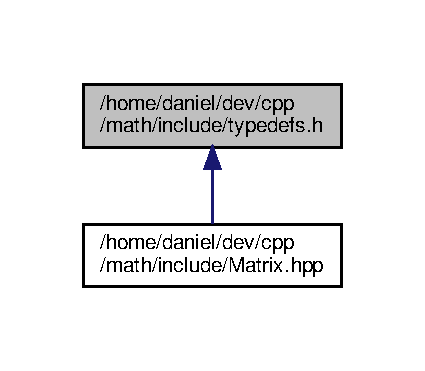
\includegraphics[width=204pt]{typedefs_8h__dep__incl}
\end{center}
\end{figure}
\subsection*{Typedefs}
\begin{DoxyCompactItemize}
\item 
typedef unsigned int \hyperlink{typedefs_8h_a7b9b9413622e67b9df7f2d090b48682b}{math\+::uint}
\item 
typedef unsigned long \hyperlink{typedefs_8h_ad71e7929690f0e5f868b5fb9b6ad36a8}{math\+::ul}
\item 
typedef unsigned long long \hyperlink{typedefs_8h_aa4f2818f8bf4329fd20d5517190a4d85}{math\+::ull}
\end{DoxyCompactItemize}


\subsection{Detailed Description}
Defines utilility types for math library. \begin{DoxyAuthor}{Author}
Daniel Nichols 
\end{DoxyAuthor}
\begin{DoxyDate}{Date}
October 2018 
\end{DoxyDate}


\subsection{Typedef Documentation}
\mbox{\Hypertarget{typedefs_8h_file_a7b9b9413622e67b9df7f2d090b48682b}\label{typedefs_8h_file_a7b9b9413622e67b9df7f2d090b48682b}} 
\index{typedefs.\+h@{typedefs.\+h}!uint@{uint}}
\index{uint@{uint}!typedefs.\+h@{typedefs.\+h}}
\subsubsection{\texorpdfstring{uint}{uint}}
{\footnotesize\ttfamily typedef unsigned int \hyperlink{typedefs_8h_a7b9b9413622e67b9df7f2d090b48682b}{math\+::uint}}

shorthand for unsigned int type \mbox{\Hypertarget{typedefs_8h_file_ad71e7929690f0e5f868b5fb9b6ad36a8}\label{typedefs_8h_file_ad71e7929690f0e5f868b5fb9b6ad36a8}} 
\index{typedefs.\+h@{typedefs.\+h}!ul@{ul}}
\index{ul@{ul}!typedefs.\+h@{typedefs.\+h}}
\subsubsection{\texorpdfstring{ul}{ul}}
{\footnotesize\ttfamily typedef unsigned long \hyperlink{typedefs_8h_ad71e7929690f0e5f868b5fb9b6ad36a8}{math\+::ul}}

shorthand for unsigned long \mbox{\Hypertarget{typedefs_8h_file_aa4f2818f8bf4329fd20d5517190a4d85}\label{typedefs_8h_file_aa4f2818f8bf4329fd20d5517190a4d85}} 
\index{typedefs.\+h@{typedefs.\+h}!ull@{ull}}
\index{ull@{ull}!typedefs.\+h@{typedefs.\+h}}
\subsubsection{\texorpdfstring{ull}{ull}}
{\footnotesize\ttfamily typedef unsigned long long \hyperlink{typedefs_8h_aa4f2818f8bf4329fd20d5517190a4d85}{math\+::ull}}

shorthand for unsigned long long 
%--- End generated contents ---

% Index
\backmatter
\newpage
\phantomsection
\clearemptydoublepage
\addcontentsline{toc}{chapter}{Index}
\printindex

\end{document}
